\chapter{Application: SASI Toy Problem}
\label{chap:application}

As mentioned at the beginning of Chapter~\ref{chap:introduction}, the simple toy model of FS~\cite{Foglizzo2009,Sato2009} was chosen as a useful initial application of our well-balanced method to the SASI. The salient details from those papers are reproduced here.

The basic set-up of the problem consists of a 2D domain with periodic boundary conditions on both edges in the $x$-direction and three distinct flow regions in the $y$-direction. First is a supersonic inflow, which is decelerated by a shock front at $y=y_\textrm{sh}$ to subsonic speeds in the second region. This is then separated from a third region (also subsonic) by a potential step at $y=y_\nabla$ which further decelerates the flow and provides a simple model of matter slowing as it nears the surface of the accreting object. Following the notation of FS, we will denote quantities in the supersonic region before the shock with a subscript `1', in the interior region between the shock and potential step with `in', and in the outflow region past the step with `out'.

A schematic view of the problem domain with all three regions can be seen on the left side of Fig.~\ref{fig:Sato1}, with the right side showing how the overall scenario is then split into two sub-problems for simulation. This separation greatly simplifies the introduction of specific advective and acoustic pertubations to appropriate locations in the interior of the domain, making it much easier to see the interactions of these disturbances at the boundaries (the shock and potential step) between the various flow regions. Overall, this provides a much simplified analogue for simulations to study the mechanisms at play during the inflow, decceleration, and accretion of matter in a collapsing star before supernova.

\begin {figure}
\centering
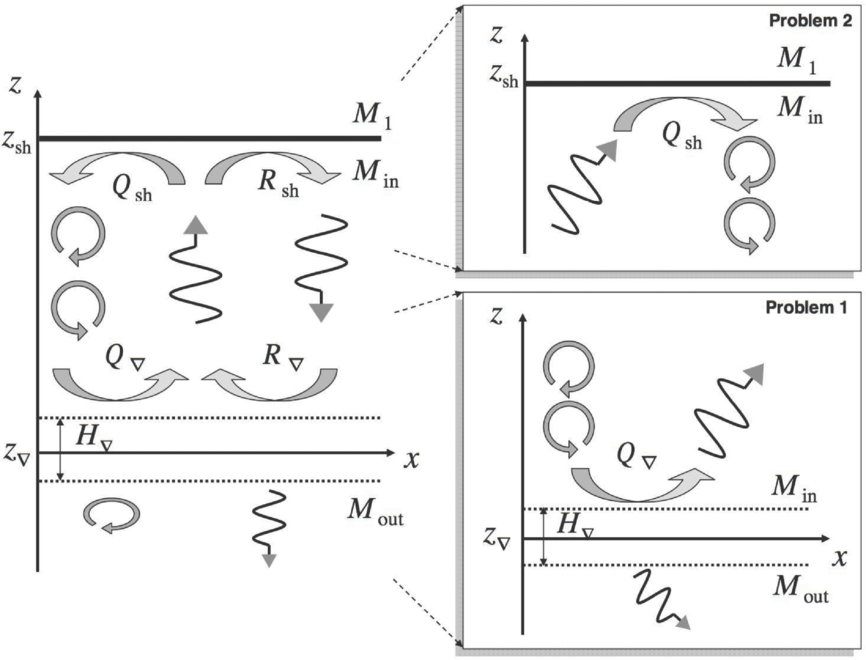
\includegraphics[width=13cm]{figures/Sato1}
\caption {This image is taken directly from FS~\cite{Sato2009}. On the left is a schematic diagram of the full toy problem for the SASI,  which is then broken into two sub-problems on the right. Circular arrows represent advective vorticity waves while wavy arrows denote acoustic pressure waves. The coupling efficiencies denote the strength of coupling between acoustic and advective waves ($Q_\textrm{sh}$, $Q_\nabla$) and the reflection of purely acoustic waves ($R_\textrm{sh}$, $R_\nabla$).}
\label{fig:Sato1}
\end{figure}

General parameters of the model problem will be presented next, followed by specific information for the potential step and stationary shock, computed separately as sub-problems 1 and 2, respectively. 


\section{Problem Set-up}
\label{sec:TP_set_up}

The general flow problem to be studied is essentially a 1D flow when at equilibrium, with the periodicity in the $x$-direction mimicking an infinitely wide flow and all variation occuring in the $y$-direction. Simulating this problem in 2D then, is done purely for studying the perturbations to this equilibrium flow, thus allowing more interesting perturbations and potential higher-dimenensional features to also be realized.

An ideal gas with an adiabatic constant $\gamma=4/3$ was simulated, the extent of the domain in the $x$-direction is denoted as $L_x$, and the entropy of the fluid is defined as
\begin{equation}
S\equiv\frac{\log\left(p/\rho^\gamma\right)}{\gamma-1}.
\end{equation}
Beginning with a Mach number of $\mathcal{M}_1=5$ at the inflow, one can then compute the relations of flow values across the shock as defined by the Rankine-Hugoniot conditions
\begin{equation}
\mathcal{M}_\textrm{in}=\sqrt{\frac{2+(\gamma-1)\mathcal{M}_1^2}{2\gamma\mathcal{M}_1^2-\gamma+1}},
\end{equation}
\begin{equation}
\frac{v_1}{v_\textrm{in}}=\frac{(\gamma+1)\mathcal{M}_1^2}{2+(\gamma-1)\mathcal{M}_1^2},
\end{equation}
\begin{equation}
\frac{\rho_1}{\rho_\textrm{in}}=\frac{v_\textrm{in}}{v_1},
\end{equation}
where $v_\textrm{in}=-\mathcal{M}_\textrm{in}c_\textrm{in}$ and the interior Mach number is found to be $\mathcal{M}_\textrm{in}=\sqrt{31/199}\approx0.39$.

A hyperbolic tangent function is used to provide a smooth step-like external potential field centred at $y_\nabla=0$ extant over a width $\approx H_\nabla$, with the exact function given by
\begin{equation}
\phi(y)=\frac{\Delta\phi}{2}\left[\tanh\left(\frac{y-y_{\nabla}}{H_{\nabla}/2}\right)+1\right],
\end{equation}
where the step size $\Delta\phi$ is set based on the ratio of the sound speeds $c_{\textrm{in}}/c_{\textrm{out}}$ in the constant regions surrounding the step, and can be computed as
\begin{equation}
\Delta\Phi=\left(\frac{\mathcal{M}_\textrm{out}^2}{2}+\frac{1}{\gamma-1}\right)c_\textrm{out}^2-\left(\frac{\mathcal{M}_\textrm{in}^2}{2}+\frac{1}{\gamma-1}\right)c_\textrm{in}^2.
\end{equation}
For all simulations, the ratio $c_\textrm{in}^2/c_\textrm{out}^2=0.75$ was used, and the step width was chosen such that $H_\nabla/H=0.1$ where $H\equiv y_\textrm{sh}-y_\nabla$ is defined to be the distance between the shock and the middle of the potential step.

A reference timescale for the advective-acoustic cycle is used to normalize the simulation times, and is calculated as
\begin{equation}
\tau_\textrm{aac}\equiv\frac{1}{1-\mathcal{M}_\textrm{in}}\frac{H}{|v_\textrm{in}|}.
\end{equation}
Units for all quantities are chosen to ensure that $c_\textrm{in}=\rho_\textrm{in}=H=1$. Using the relation $p=\rho c^2/\gamma$ we can compute the other primitive values in the interior region as $p_\textrm{in}=0.75$ and $T_\textrm{in}=1.05$ and the reference timescale as $\tau_\textrm{aac}\approx4.2$. A wavenumber $k_x=2\pi/L_x$ is used to define linear perturbations of the flow, where $L_x=4$, along with a temporal frequency defined as $\omega_0=4\pi/\tau_\textrm{aac}$.

For both sub-problems a $4\times4$ square domain is used, divided into a uniform number $N_x=N_y=400$ of square grid cells in both dimensions. This gives a uniform grid spacing of $\Delta x=\Delta y=10^{-2}$.

\subsection{Sub-Problem 1: Potential Step}
\label{subsec:sub_problem_1}

For the first sub-problem, the potential step positioned at $y_\nabla=0$ is the only flow feature simulated on a square domain defined on $y\in[-1,3]$, $x\in[0,4]$. Inflow occurs at the upper $y=3$ boundary, defined using Dirichlet conditions, and zero-gradient conditions are imposed at the $y=-1$ outflow boundary. Initial conditions are determined by computing the equilibrium flow for the given inlet primitive values over the potential field. By defining also a veritcal wavenumber $k_y=\omega_0/v_\textrm{in}$ the perturbations injected at the inlet are given by the equations
\begin{equation}
\delta S\equiv\epsilon_S\cos\left(-\omega_0t+k_xx+k_yy\right),
\end{equation}
\begin{equation}
\frac{\delta \rho}{\rho_\textrm{in}}\equiv\exp\left(-\frac{\gamma-1}{\gamma}\delta S\right)-1,
\end{equation}
where $\epsilon_S=10^{-3}$ is the amplitiude of the generated entropy waves.

These incoming waves are desired to be at pressure equilibrium ($\delta p=0$), and so from the equation of state one can then determine the consistent temperature perturbation
\begin{equation}
\frac{\delta T}{T_\textrm{in}}=\left(1+\frac{\delta\rho}{\rho_\textrm{in}}\right)^{-1}-1=\exp\left(\frac{\gamma-1}{\gamma}\delta S\right)-1.
\end{equation}
Deviations to the 2D velocity components are given as
\begin{equation}
\delta v_x\equiv\frac{k_x\omega_0c_\textrm{in}^2}{\omega_0^2+k_x^2v_\textrm{in}^2}\frac{\delta S}{\gamma} \quad \textrm{and} \quad \delta v_y\equiv\frac{k_x^2v_\textrm{in}c_\textrm{in}^2}{\omega_0^2+k_x^2v_\textrm{in}^2}\frac{\delta S}{\gamma},
\end{equation}
which result in the generation of the following vorticity waves 
\begin{equation}
\delta w_y=-\frac{k_xc_\textrm{in}^2}{v_\textrm{in}}\frac{\epsilon_S}{\gamma}\sin\left(-\omega_0t+k_xx+k_yy\right).
\end{equation}
These waves, which are injected only at the inlet, are allowed to travel through the interior region towards the potential step, and then any resultant coupling of the vorticity waves into reflected pressure waves is observed.

\subsection{Sub-Problem 2: Standing Shock}
\label{subsec:sub_problem_2}

For the second sub-problem, only the shock front positioned at $y_\textrm{sh}=1$ is simulated, with the square domain now defined on $y\in[-2,2]$, $x\in[0,4]$. Inflow is now supersonic and again set with Dirichlet boundaries at $y=2$, although the outflow conditions at $y=-2$ are different from sub-problem 1. Homogoneous Neumann conditions are still used initially while no perturbations are present in the system, to allow the shock to ``settle in'' and any waves generated by this process to propagate cleanly out of the system. Once a steady state is reached, however, the outflow conditions are changed to be also Dirichlet in order to inject the desired perturbations into the domain from the outflow boundary. Initial conditions are in this case determined purely by the Rankine-Hugoniot conditions given earlier to define the shock, since the potential field is now constant throughout the entire domain.

Voriticity free pressure perturbations are generated for this sub-problem, and by defining a new vertical wavenumber
\begin{equation}
k_y^\pm=\frac{\omega}{c_\textrm{in}}\frac{\mathcal{M}_\textrm{in}\mp\mu}{1-\mathcal{M}_\textrm{in}^2},
\end{equation}
and density perturbation amplitude $\epsilon_\rho=10^{-3}$, one has the equations for the outlet perturbations as
\begin{align}
\frac{\delta\rho}{\rho_\textrm{in}}&\equiv\left(\frac{1+\mu\mathcal{M}_\textrm{in}}{1-\mathcal{M}_\textrm{in}^2}\right)\epsilon_\rho\cos\left(-\omega_0t+k_xx+k_y^-y\right), \\
\frac{\delta p}{p_\textrm{in}}&\equiv\left(1+\frac{\delta\rho}{\rho_\textrm{in}}\right)^\gamma-1,
\end{align}
where one can again use the equation of state to determine the consistent temperature deviation
\begin{equation}
\frac{\delta T}{T_\textrm{in}}=\left(1+\frac{\delta\rho}{\rho_\textrm{in}}\right)^{\gamma-1}-1.
\end{equation}
Velocity perturbations for these purely acoustic pressure waves are given by
\begin{align}
\delta v_x&\equiv\left(\frac{k_xc_\textrm{in}^2}{\omega_0}\right)\epsilon_\rho\cos\left(-\omega_0t+k_xx+k_y^-y\right), \\
\delta v_y&\equiv\left(\frac{\mu+\mathcal{M}_\textrm{in}}{1-\mathcal{M}_\textrm{in}^2}c_\textrm{in}\right)\epsilon_\rho\cos\left(-\omega_0t+k_xx+k_y^-y\right),
\end{align}
where the parameter $\mu$ is simply used for convenience and expands as
\begin{equation}
\mu\equiv\sqrt{1-\frac{k_x^2c_\textrm{in}^2}{\omega_0^2}\left(1-\mathcal{M}_\textrm{in}^2\right)}.
\end{equation}
These waves then propagate towards the shock front, and any resultant generation of reflected vorticity waves is measured.
